%% LyX 2.1.4 created this file.  For more info, see http://www.lyx.org/.
%% Do not edit unless you really know what you are doing.
\documentclass[a4paper,oneside,brazil,11pt,a4paper,openright,titlepage,usenames,dvipsnames]{book}
\usepackage[utf8]{inputenc}
\usepackage[T1]{fontenc}
\usepackage{lmodern}
\setcounter{secnumdepth}{3}
\setcounter{tocdepth}{3}
\usepackage{array}
\usepackage{verbatim}
\usepackage{calc}
\usepackage{textcomp}
\usepackage{amssymb}
\usepackage{graphicx}

\makeatletter

%%%%%%%%%%%%%%%%%%%%%%%%%%%%%% LyX specific LaTeX commands.
\pdfpageheight\paperheight
\pdfpagewidth\paperwidth

%% Because html converters don't know tabularnewline
\providecommand{\tabularnewline}{\\}

%%%%%%%%%%%%%%%%%%%%%%%%%%%%%% User specified LaTeX commands.
% Classe alternativa, apropriada para impressão frente-verso. Inclui páginas em branco
% de forma que capítulos sempre tenham início na página à direita:
% \documentclass[11pt,a4paper,openright,titlepage]{book}

% Pacotes
\usepackage[T1]{fontenc}
\usepackage[brazilian]{babel}
\usepackage{epsfig}
\usepackage{subfigure}
\usepackage{amsfonts}
\usepackage{amsmath}
\usepackage[thmmarks,amsmath]{ntheorem}%\usepackage{amsthm}
\usepackage{boxedminipage}
\usepackage{geometry}
\usepackage{theorem}
\usepackage{fancybox}
\usepackage{fancyhdr}
\usepackage{ifthen}
\usepackage{url}
\usepackage{afterpage}
\usepackage{color}
\usepackage{colortbl}
\usepackage{rotating}
\usepackage{makeidx}
\usepackage{indentfirst}
% Pacotes para adição de figuras do inkscape
\usepackage{graphicx}
\usepackage{import}

% Escolher um dos seguintes formatos:
\usepackage{ft2unb} % segue padrão de fontes do Latex

\makeindex

\makeatother

\usepackage{babel}
\begin{document}
\setcounter{secnumdepth}{3}
\setcounter{tocdepth}{2}
\pagestyle{empty}

\grau{Engenheiro de Controle e Automação}

\tipodemonografia{RELATÓRIO DE PROGRESSO\\TRABALHO DE GRADUAÇÃO 1}

\begin{comment}
Título
\end{comment}


\titulolinhai{INTELIGÊNCIA COMPUTACIONAL}

\titulolinhaii{PARA FUTEBOL DE ROBÔS MULTI-AGENTE}

\titulolinhaiii{}

\titulolinhaiv{}

\begin{comment}
Autores. Basta retirar o texto totalmente caso não haja um determinado
autor.
\end{comment}


\autori{Bruno Andreghetti Dantas}

\autorii{Samuel Venzi Lima Monteiro de Oliveira}

\autoriii{}

\begin{comment}
Membros da banca. Basta retirar o texto totalmente caso não haja um
determinado membro da banca.
\end{comment}


\membrodabancai{}

\membrodabancaifuncao{}

\membrodabancaii{}

\membrodabancaiifuncao{o}

\membrodabancaiii{}

\membrodabancaiiifuncao{}

\membrodabancaiv{}

\membrodabancaivfuncao{}

\membrodabancav{}

\membrodabancavfuncao{}

\begin{comment}
Data de defesa: mês e ano
\end{comment}

\mes{dezembro}
\ano{2019}

\begin{comment}
Comandos para criar a capa e a página de assinaturas
\end{comment}


\capaprincipal
% \capaassinaturas

\begin{comment}
Ficha Catalográfica
\end{comment}




\begin{comment}
Dedicatória
\end{comment}


% \frontmatter

\begin{comment}
Texto de dedicatória do primeiro autor.
\end{comment}


% \dedicatoriaautori{um beijo pra minha mãe, pro meu pai, e pra você}

\begin{comment}
Texto de dedicatória do segundo autor. Caso não tenha um segundo autor,
este texto não será mostrado
\end{comment}


% \dedicatoriaautorii{Dedicatória do autor 2}

\begin{comment}
Texto de dedicatória do terceiro autor. Caso não tenha um terceiro
autor, este texto não será mostrado
\end{comment}


% \dedicatoriaautoriii{Dedicatória do autor 3}

\begin{comment}
Comando para criar a página de dedicatória
\end{comment}


% \dedicatoria

\begin{comment}
Agradecimentos
\end{comment}


\begin{comment}
Texto de agradecimentos do primeiro autor.
\end{comment}


\agradecimentosautori{Agradecimentos!}

\begin{comment}
Texto de agradecimentos do segundo autor. Caso não tenha um segundo
autor, este texto não será mostrado.
\end{comment}


\agradecimentosautorii{A inclusão desta seção de agradecimentos é
opcional e fica à critério do(s) autor(es), que caso deseje(em) inclui-la
deverá(ão) utilizar este espaço, seguindo esta formatação.}

\begin{comment}
Texto de agradecimentos do terceiro autor. Caso não tenha um terceiro
autor, este texto não será mostrado.
\end{comment}


\agradecimentosautoriii{A inclusão desta seção de agradecimentos
é opcional e fica à critério do(s) autor(es), que caso deseje(em)
inclui-la deverá(ão) utilizar este espaço, seguindo esta formatação.}

\begin{comment}
Comando para criar a página de agradecimentos
\end{comment}


% \agradecimentos

% \resumo{resumo}{Resumo!

% \medskip{}


% Palavras Chave: bla, ble, bli

% }\vspace*{2cm}


% \resumo{Abstract}{Abstract, in English ofc!

% \medskip{}


% Keywords: bla, ble, bli

% }

\begin{comment}
Listas de conteúdo, figuras e tabelas
\end{comment}


\sumario
% \listadefiguras
% \listadetabelas

\begin{comment}
Lista de Símbolos
\end{comment}


% %TCIDATA{LaTeXparent=0,0,these.tex}


%\chapter*{\setfontarial\mdseries LISTA DE SÍMBOLOS} % se usar ft1unb.sty, descomente esta linha



\chapter*{LISTA DE SÍMBOLOS}

% se usar ft2unb.sty, descomente esta linha



\subsection*{Símbolos Latinos}

\begin{tabular}{p{0.1\textwidth}p{0.63\textwidth}>{\PreserveBacklash\raggedleft}p{0.15\textwidth}}
$v$  & Velocidade linear  & {[}m/s{]}\tabularnewline
\end{tabular}


\subsection*{Símbolos Gregos}

\begin{tabular}{p{0.1\textwidth}p{0.63\textwidth}>{\PreserveBacklash\raggedleft}p{0.15\textwidth}}
$\omega$ & Velocidade angular & {[}rad/s{]}\tabularnewline
\end{tabular}


\subsection*{Grupos Adimensionais}

\begin{tabular}{p{0.1\textwidth}p{0.8\textwidth}}
i, k & Contador\tabularnewline
\end{tabular}


\subsection*{Subscritos}

\begin{tabular}{p{0.1\textwidth}p{0.8\textwidth}}
$ref$  & referência \tabularnewline
$fer$  & ferramenta \tabularnewline
$sis$  & sistema \tabularnewline
$des$  & desejado\tabularnewline
\end{tabular}


\subsection*{Sobrescritos}

\begin{tabular}{p{0.1\textwidth}p{0.8\textwidth}}
$\cdot$  & Variação temporal \tabularnewline
$-$  & Valor médio \tabularnewline
\end{tabular}


\subsection*{Siglas}

\begin{tabular}{p{0.1\textwidth}p{0.8\textwidth}}
PCI  & \textit{Peripheral Component Interconnect}\tabularnewline
CPU & Unidade Central de Processamento - \textit{Central Processing Unit} \tabularnewline
AO & Saída Analógica - \textit{Analog Out}\tabularnewline
DO & Saída Digital - \textit{Digital Out}\tabularnewline
CS & Seletor de \textit{Chip - Chip Select}\tabularnewline
SC & Sem Conexão\tabularnewline
P.I. & Placa de Interface\tabularnewline
ICW & \textit{Initialization Command Words}\tabularnewline
OCW & \textit{Operational Control Word}\tabularnewline
\end{tabular}


\begin{comment}
Corpo Principal
\end{comment}


\mainmatter
\setcounter{page}{1}
\pagenumbering{arabic}
\pagestyle{plain}

\begin{comment}
Introdução 
\end{comment}

\chapter{Introdução}

\label{CapIntro}

% Resumo opcional. Comentar se não usar.
% \resumodocapitulo{Resumo opcional}


\section{RoboCup Soccer Simulation 2D}
\par A ideia de robôs jogando futebol foi proposta pela primeira vez em 1992 por Alan Mackworth\cite{mackworth1993seeing}.
Desde então a comunidade científica tem criado iniciativas buscando por soluções que tornem isso realidade.
Uma delas é a \textit{Robot World Cup Initiative}, abreviada como \textit{RoboCup}, que teve sua primeira edição em 1997 com mais de 40 equipes distribuídas entre as diversas categorias do evento.
\par O objetivo da iniciativa, definido pela \textit{RoboCup Federation}, é que por volta da metade do século XXI, um time de robôs humanóides autônomos vençam uma partida contra os campeões da Copa do Mundo mais recente. Mesmo que o objetivo pareça ambicioso, ele guia as pesquisas e motiva o avanço no campo.
Atualmente, a RoboCup conta com mais de 10 categorias, entre elas a \textit{RoboCup Soccer Simulation 2D}, abreviada RCSS, objeto de estudo deste projeto.
\par A categoria apresenta, também, grande relevância no cenário brasileiro.
Desde 2005, a RCSS está presente na maior competição de robótica da América Latina, a \textit{Latin American Robotics Competition}, LARC.
\par Nessa categoria, duas equipes de 11 jogadores autônomos e independentes jogam futebol em um ambiente virtual bidimensional.
Um servidor é responsável por esse ambiente e possui informação absoluta sobre o estado do jogo e suas regras.
Os jogadores, por sua vez, recebem dele informação incompleta e ruidosa de seus sensores virtuais, podendo executar comandos a fim de atuar sobre o estado do jogo.

\subsection{Servidor da partida}
\par Um servidor que executa a partida é disponibilizado pelos organizadores da competição e este pode ser utilizado, também, para desenvolvimento. O servidor, portanto, apresenta, internamente, algumas das regras da partida bem como um juiz autônomo que age para determinar gols, faltas e demais situações de uma partida de futebol. Caso necessário, um juiz humano poderá intervir em situações não contempladas pelas regras do servidor.
\par O servidor simula todos os movimentos e ações dos jogadores e da bola. Clientes externos se conectam ao servidor e cada cliente controla um único jogador. A comunição entre o cliente e o servidor é feita a partir do protocolo UDP por meio de mensagens com sintaxe específica e definida pelo servidor.
\par De forma a permitir o acompanhamento visual da partida, um monitor também é disponibilizado, porém não é necessário para que uma partida ocorra com sucesso.
\par O servidor, ainda, possui o modo \textit{trainer} para utilização durante treinamentos de algoritmos de inteligência computacional. Este modo permite a conexão de um cliente do tipo treinador que tem acesso absoluto às informações da partida e pode mudar modos de jogo e ainda mover arbitrariamente jogadores e bola. Adicionalmente, é possível acelerar os ciclos da partida permitindo o treinamento em tempo hábil.

\begin{figure}[h]
	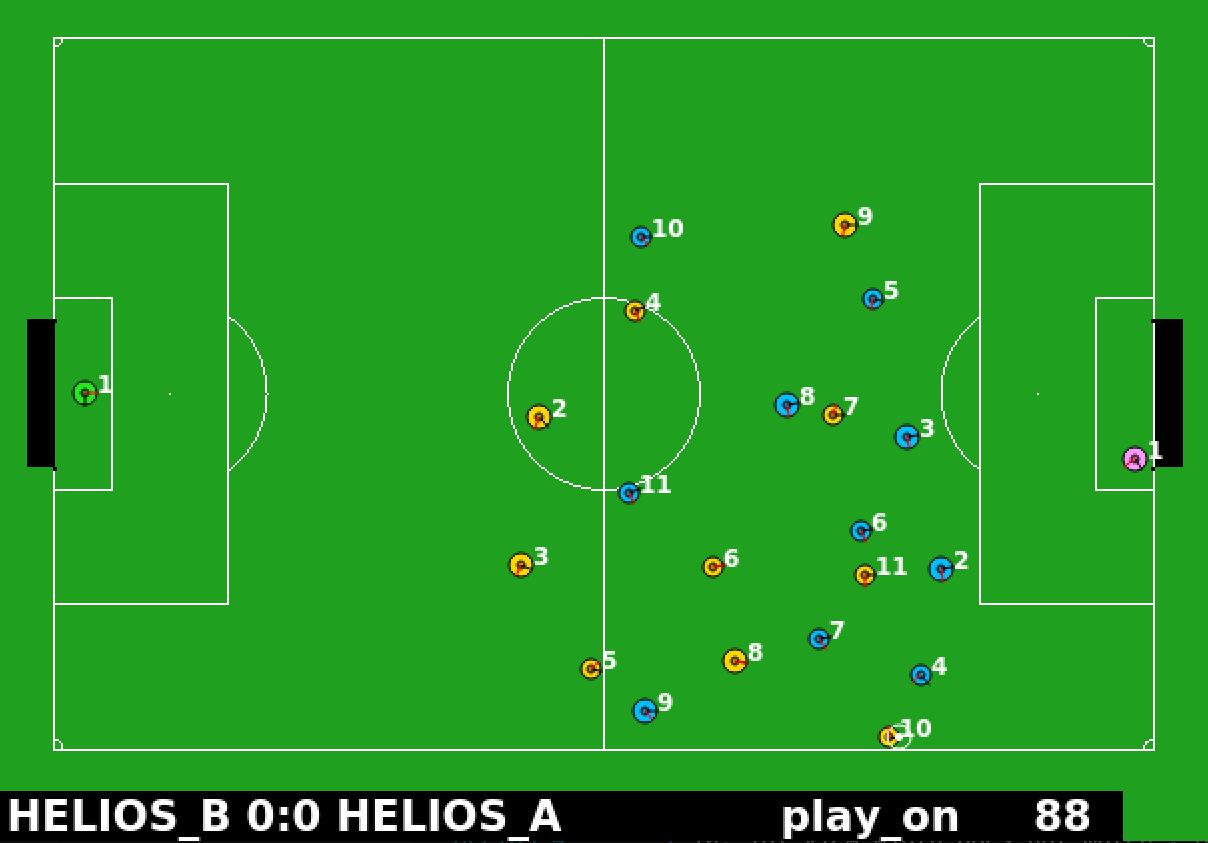
\includegraphics[width=0.7\linewidth]{figs/server.png}
	\centering
	\caption{Visualização de uma partida em andamento}
	\label{fig:rcssserver}
\end{figure}

\subsection{Cliente}
\par Os jogadores são controlados por clientes externos conectados ao servidor. Como já foi dito, um cliente corresponde a um único jogador e os clientes só podem ser comunicar com mensagens mandadas através do servidor da partida.
\par O cliente pode ser desenvolvido em qualquer linguagem desde que se comunique com o servidor pelo protolo UDP e utilize a sintaxe de mensagens reconhecida pelo sistema. Há várias escolhas disponíveis para a construção do cliente, sendo decisão de cada equipe competidora como fazê-lo.

\subsection{Sensores}

Para receber informações a respeito da situação do jogo, cada cliente conectado recebe mensagens referentes a atualizações de três sensores virtuais descritos abaixo.

\subsubsection{Sensor Auditivo}

As mensagens do sensor auditivo são do seguinte formato:

\textit{(hear Tempo Remetente "mensagem")}

Onde \textit{Tempo} é o número do ciclo em que a mensagem foi ouvida e \textit{Remetente} é descrição de quem enviou a mensagem. O \textit{Remetente} pode ser o árbitro, outros jogadores, um dos treinadores ou o próprio jogador.

No escopo deste trabalho, apenas as mensagens do árbitro serão consideradas, não sendo implementada nenhuma forma de comunicação direta entre os jogadores.

\subsubsection{Sensor Visual}

% TODO

\subsubsection{Sensor Corporal}

% TODO

\subsection{Ações}

% TODO

\section{Abordagens utilizadas na categoria}
\par Uma pesquisa sobre as abordagens para o desenvolvimento das estratégias dos times participantes da RCSS revelou o uso recorrente de métodos de inteligência computacional.
\par A equipe chinesa \textit{WrightEagle}, campeã do principal evento internacional da categoria diversas vezes, utiliza Processos de Decisão de Markov ou MDPs para modelar a partida\cite{bai2015online}.
\par A equipe japonesa \textit{HELIOS}, campeã de 2018 da categoria na RoboCup, divide seus jogadores em categorias "chutadores" e "não-chutadores".
Os chutadores são responsáveis por realizar o planejamento de sequência de ações, utilizando métodos de valor de ação.
Os não-chutadores, por sua vez, não tem conhecimento do planejamento feito pelos chutadores, e devem obter o máximo de informações relevantes para tentar gerar a mesma sequência de ações que jogador chutador\cite{nakashima2018helios2018}.
\par A equipe brasileira \textit{ITAndroids}, atual campeã da LARC, utiliza a abordagem de sequência de ações, similar à \textit{HELIOS}, explorando uma árvore de ações criada dinamicamente de forma a maximizar o valor de cada ação. Além disso, utilizam Otimização por Enxame de Partículas \cite{melloitandroids} para adequar os parâmetros que calculam o valor da ação. A \textit{ITAndroids} também vem desenvolvendo o uso de Aprendizagem por Reforço Profunda \cite{maximoitandroids}.
\par Muitas equipes, ainda, desenvolvem seus agentes utilizando o agente base da equipe \textit{HELIOS}, \textit{Agent2d} com a biblioteca \textit{Librcsc}, escritas em C++. Por isso, é comum que haja semelhança na construção dos agentes dessas equipes.


\begin{comment}
Fundamentos
\end{comment}
\chapter{Fundamentação Teórica \label{chap:FundamentacaoMatematica}}

% Resumo opcional. Comentar se não usar.
% \resumodocapitulo{Resumo opcional.}


\section{Processos de Decisão de Markov}

O problema abordado neste trabalho pode ser descrito como um Processo de Decisão de Markov (MDP).
MDP é uma forma clássica de representação matemática de processos de decisão sequenciais.
Nessa representação, cada ação tomada por um agente que interage com o ambiente transforma o estado do processo e determina a recompensa que o agente recebe imediatamente.
Esse estado também deve ser suficiente para conter toda a informação relevante para a dinâmica futura do processo.

\begin{figure}[h]
	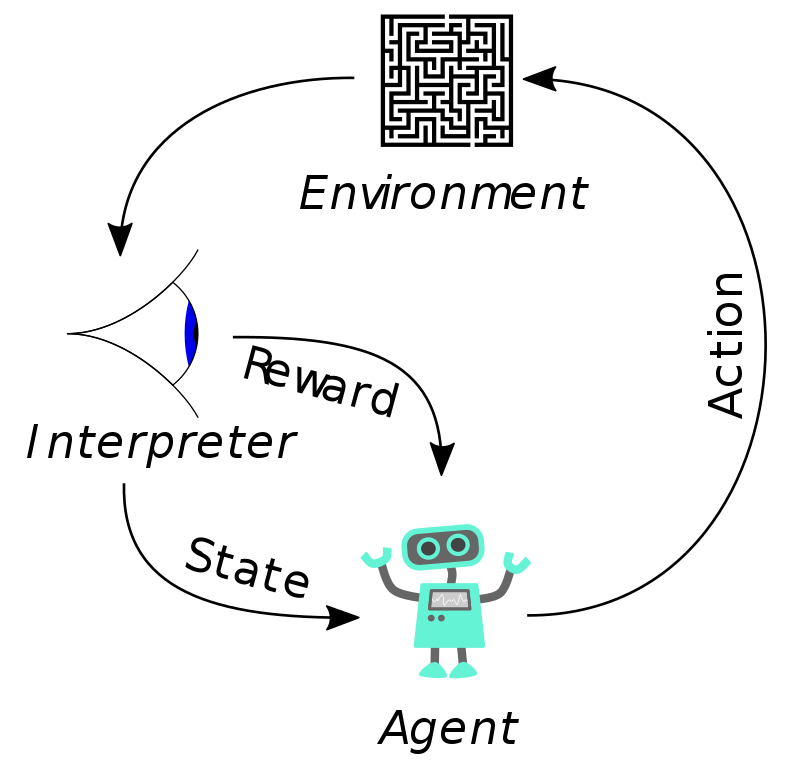
\includegraphics[width=0.6\linewidth]{figs/RL.png}
	\centering
	\caption{Interação agente-ambiente em um MDP \cite{sutton2018reinforcement}.} % figure 3.1 page 48
	\label{fig:mdp_env}
\end{figure}

Assim, dado um espaço de estados $\mathcal{S}$, um espaço de ações $\mathcal{A}$ e um espaço de recompensas $\mathcal{R}$, para cada par $(S, A)$ com $S \in \mathcal{S}$ sendo o estado atual do processo e $A \in \mathcal{A}$ a ação tomada pelo agente existe uma determinada probabilidade de atingir o estado $S' \in \mathcal{S}$ e receber a recompensa imediata $R \in \mathcal{R}$ \cite{sutton2018reinforcement}.

Essa abordagem é bastante flexível e torna possível a modelagem da dinâmica do futebol virtual de robôs de diversas maneiras de modo que cada agente possa construir um estado percebido a partir de seus sensores e tomar decisões acerca de qual ação tomar diante desse estado a fim de maximizar a recompensa recebida.

\subsection{MDP Episódico e Contínuo}

Um MDP pode ser caracterizado quanto à presença de um estado terminal. Caso o MDP tenha um ou mais estados que determinem o fim do processo, ele é dito episódico. A simulação de futebol de robôs tratada neste trabalho é um exemplo de MDP episódico, uma vez que o MDP termina ao se encerrar o tempo de jogo.

Em contrapartida, há MDPs onde não está bem definido nenhum estado terminal. Nesses casos, o MDP pode continuar indefinidamente até que uma ação externa ao MDP determine a sua parada. Um exemplo disso é um MDP que controle um robô numa linha de produção. Caso o sistema de automação supervisor desse robô não determine sua parada (por falta de insumos, por exemplo), o MDP pode seguir operando indefinidamente.

Nesta fundamentação, será tratado com mais atenção o caso episódico uma vez que é o caso que interessa para aplicação na simulação de futebol de robôs.

\subsection{Recompensa e Retorno}

Como definido acima, para cada ação tomada em um MDP é atribuída uma recompensa $R \in \mathcal{R}$. Essa recompensa é sempre referente ao instante de tempo anterior, ou seja, não depende de qualquer outro fator que não o par $(S_t, A_t)$ executados no instante $t$ e a função de probabilidade associada pelo MDP a esse par. Por isso, é comum utilizar a notação $R_{t+1}$ para se referir à recompensa obtida após tomar a ação $A_t$ no instante de tempo $t$.

Porém em muitos casos é esperado de um agente que ele tome decisões que maximizem a recompensa total ao fim de um episódio, ou seja, é esperado que se escolha $A_t$ a fim de maximizar não apenas $R_{t+1}$ mas sim o retorno $G_{t+1} = R_{t+1} + R_{t+2} + \dotsc + R_{terminal}$.

\subsection{Políticas}

É dado o nome de política para qualquer função $\pi(S) \to \mathcal{A}$ que leve de um estado qualquer do MDP para uma ação a ser tomada. Para cada política $\pi$, existe uma função $q_\pi(S, A)$ que, para cada par de estado e ação, define a esperança de retorno caso o agente continue seguindo a política $\pi$ no restante do episódio.

É possível comparar duas políticas $\pi$ e $\pi'$ a respeito de suas funções $q$. A política $\pi$ é considerada melhor ou igual a $\pi$, ou $\pi \ge \pi'$, caso $q_\pi(S, A) \ge q_{\pi'}(S, A)$ para todo par $(S, A)$.

Sempre há ao menos uma política melhor ou igual a todas as outras, denominada política ótima. Qualquer política que cumpra esse requisito é denominada $\pi_*$ e, caso haja mais de uma, todas devem possuir a mesma função $q$ denominada $q_*$ \cite{sutton2018reinforcement}. % chap 3.6

Uma política que toma sempre o caminho de maior retorno é denominada gulosa, e uma política que toma o caminho de maior retorno mas escolhe uma ação aleatoriamente com probabilidade parametrizada $\epsilon$ é denominada $\epsilon$-gulosa.

\section{Aprendizagem por Reforço}

Dada uma modelagem do problema como um MDP, resta obter uma maneira de estimar as probabilidades que determinam a dinâmica desse MDP, e com isso determinar um critério de decisão - denominado política - capaz de maximizar a recompensa a longo prazo recebida pelo agente.

O conjunto de técnicas que resolvem esse tipo de problema é chamado de Aprendizagem por Reforço.
No campo da aprendizagem de máquina, ela se difere da Aprendizagem Supervisionada por não haver um conjunto de pares $(s, a)$ dados como corretos.
Nesse tipo de aprendizagem, o objetivo é extrapolar uma solução genérica a partir de exemplos de um conjunto de treinamento dado como correto, o que não é prático em problemas em que não se tem exemplos de comportamentos corretos e que representem bem o conjunto total de situações possíveis.
Ela também se diferencia da Aprendizagem Não-Supervisionada, que tradicionalmente visa encontrar estrutura em conjuntos de dados não classificados, enquanto a Aprendizagem por Reforço visa maximizar um sinal de recompensa \cite{sutton2018reinforcement}.

Desse modo, as técnicas de Aprendizagem por Reforço serão aplicadas a fim de buscar políticas capazes de maximizar o desempenho dos jogadores virtuais, ou seja, obter políticas que tornem os agentes capazes de fazer gols e evitar que os jogadores do time adversário façam gols.

\subsection{Aprendizagem On-policy e Off-policy}

Entre as técnicas de aprendizagem por reforço existe uma divisão entre a aprendizagem on-policy e a aprendizagem off-policy, referentes à relação entre a política executada durante o aprendizado e a política sobre a qual se quer aprender.

Nos algoritmos de aprendizagem on-policy, o agente aprende a respeito da política $\pi$ enquanto navega o MDP de acordo com a própria política $\pi$.

Já nos algoritmos de aprendizagem off-policy, o agente aprende a respeito da política alvo $\pi$ enquanto navega o MDP de acordo com a política $b$, ou seja, ele estima a função $q_{\pi}$ enquanto segue a política $b$.

Os métodos off-policy costumam introduzir variância no processo, tornando o aprendizado ruidoso e em alguns casos a garantia de convergência é provada apenas para o caso on-policy. % TODO: carece de fonte

Além disso, é possível observar que a aprendizagem on-policy é apenas um caso particular da aprendizagem off-policy em que $b = \pi$.

\subsection{Soluções Tabulares e Aproximadas}

A maioria dos métodos de aprendizagem por reforço são testados e validados em MDPs cujos espaços de estados $\mathcal{S}$ e de ações $\mathcal{A}$ são suficientemente pequenos. Para esses MDPs é possível utilizar uma solução tabular, ou seja, a função $Q$ poda ser armazenada em uma tabela de tamanho razoável e sua imagem para cada par estado-ação pode ser atualizado individualmente.

Infelizmente, em diversas aplicações a quantidade de estados possíveis é grande demais ou até mesmo infinito, como é o caso de sistemas em que determinada característica do estado é medida como uma grandeza contínua. Nesses casos, é impossível esperar que se obtenha soluções ótimas mesmo com tempo infinito, portanto o objetivo é obter uma solução aproximada que seja boa o suficiente para a aplicação desejada.

A ferramenta matemática utilizada para viabilizar soluções aproximadas é o conceito de aproximadores de função, muito utilizados na aprendizagem supervisionada. Entre os aproximadores mais utilizados estão os aproximadores lineares e as redes neurais multicamada.

Neste trabalho serão utilizados métodos de solução aproximada devido à grande quantidade de informações simultâneas às quais o jogador tem acesso.

\subsection{Q-Learning}

Um dos algoritmos mais populares no campo da aprendizagem por reforço é o Q-Learning. Trata-se de um método off-policy que aproxima diretamente a função $q_*$ independente da política que estiver sendo adotada pelo agente durante o treinamento.

O algoritmo é também muito simples. Dada uma representação tabular $Q: (\mathcal{S},\mathcal{A}) \to \mathbb{R}$ da função $q_*$, para cada instante de tempo $t$ é realizada a seguinte atualização a fim de aproximar $Q$ de $q_*$:

\begin{equation}
Q(S_t, A_t) \leftarrow Q(S_t, A_t) + \alpha[R_{t+1} + \max_{a} Q(S_{t+1}, a) - Q(S_t, A_t)]
\end{equation}

Após iterações suficientes, espera-se que $Q$ convirja para $q_*$. Em alguns casos a convergência é provada matematicamente.

Uma vez estimada a função $q_*$, é simples obter a política ótima. Basta escolher a ação que maximiza $q_*$ no estado atual, ou seja:

\begin{equation}
A_{t+1} = \max_{a} q_*(S_t, a)
\end{equation}

É comum, mas não obrigatório, que a política $b$ seguida durante o aprendizado seja $epsilon$-gulosa em relação à aproximação Q.

\subsection{Q-Learning Duplo}

Apesar de popular o Q-Learning possui um problema de viés de maximização. Uma vez que a aproximação $Q$ é imprecisa no início do treinamento, é possível que o retorno esperado estimado seja enviesado para um valor maior do que o real.

Como solução para esse problema, é utilizada a abordagem do Q-Learning Duplo. Nela são utilizadas duas aproximações, $Q_1$ e $Q_2$, e a atualização de $Q$ é dada da seguinte forma:

\begin{equation}
\label{eq:doubleq}
Q_1(S_t, A_t) \leftarrow Q_1(S_t, A_t) + \alpha[R_{t+1} + Q_2(S_{t+1}, \text{arg}\max_a Q_1(S_{t+1}, a)) - Q_1(S_t, A_t)]
\end{equation}

Em metade das iterações (através de um sorteio, por exemplo), as aproximações $Q_1$ e $Q_2$ são trocadas. Com isso é anulado o viés de maximização gerado pelo uso de $\max_a Q$ como estimativa de retorno para os estados seguintes.

A vantagem desse método é que apesar de dobrar os requisitos de memória do algoritmo, afinal será preciso armazenar os dados referentes a duas aproximaçoes, ele não aumenta o custo computacional por iteração.


\begin{comment}
Desenvolvimento
\end{comment}
\chapter{Desenvolvimento \label{chap:Desenvolvimento}}

% Resumo opcional. Comentar se não usar.
% \resumodocapitulo{Resumo opcional.}


\section{Biblioteca}
\par O servidor da partida apresenta, como já mencionado, um protocolo de comunicação e sintaxe de mensagens específica. Uma biblioteca de interfaceamento é proposta com o objetivo de abstrair os detalhes de comunicação de construção de mensagens e facilitar, assim, o desenvolvimento dos programas jogadores. Esta abordagem já é comum na categoria e existem soluções de código aberto como a \textit{librcsc}, utilizada por várias equipes, usualmente atreladas ao agente base \textit{agent2d}, desenvolvidas pela equipe \textit{HELIOS}.

\par Uma biblioteca própria desenvolvida em linguagem Go é proposta como forma de modernização e diversificação da base de código utilizada pelas equipes.

\section{Agente Único}
\par Inicialmente, deseja-se realizar o treinamento de um agente único que, com as informações de seus sensores, consiga com sucesso levar a bola ao gol. Essa proposta tem como objetivo fundamentar os conhecimentos e validar a base de código para a realização de um treinamento de um time de múltiplos agentes em um estágio posterior.
\par O desenvolvimento de um agente único, inicialmente, permite adquirir o entendimento necessário para a definição do vetor de estados e ajuste das técnicas de treinamento. Além disso, busca-se uma maior agilidade na substituição e teste na estrutura do vetor de estados e no algoritmo de treinamento, uma vez que o custo computacional deste cenário é consideravelmente menor que o custo do treinamento de um time completo.

% \subsection{Vetor de Estados} % não sei se faz sentido, sendo que não temos quase nada pronto sobre isso

\section{Agentes Concorrentes}

Após validação do sistema com agente único, é interessante experimentar com treinamento adversarial de apenas 2 jogadores em formato um-contra-um. A intenção dessa etapa é experimentar com o sistema o caso adversarial, no qual há um ou mais agentes com objetivo oposto ao do agente sendo treinado.

\section{Múltiplos Agentes}

Após validar os casos de agente único e de agentes concorrentes, propõe-se um treinamento completo em jogos 11 contra 11. O objetivo é, ao final do processo, termos um time capaz de jogar contra os principais times da atualidade na categoria RoboCup Soccer Simulation 2D.

Para isso, os agentes devem ser capazes de cooperar e reagir aos movimentos da equipe oposta a fim de marcar gols e evitar os gols do adversário.

% \subsection{Vetor de Estados}




\begin{comment}
Conclusões
\end{comment}

\chapter{Conclusões}

\label{CapConclusoes}


\section{Reimplementação da Interface com o Servidor}

\section{Treinamento de uma Equipe para Participação em Competições}

 

\begin{comment}
Bibliografia
\end{comment}


\renewcommand{\bibname}{REFERÊNCIAS BIBLIOGRÁFICAS}
\addcontentsline{toc}{chapter}{REFERÊNCIAS BIBLIOGRÁFICAS}

\bibliographystyle{abnt-num}
\bibliography{bibliography}


\begin{comment}
Anexos
\end{comment}


% \anexos
\makeatletter
% não retirar estes comandos
\renewcommand{\@makechapterhead}[1]{%
  {\parindent \z@ \raggedleft \setfontarial\bfseries
\LARGE \thechapter. \space\space
\uppercase{#1}\par
\vskip 40\p@
}
}
\makeatother

\begin{comment}
Anexo I: Descrição do CD
\end{comment}


% 
\chapter{Descrição do conteúdo do CD}

\label{AnCD}

Descrever CD.


% \refstepcounter{noAnexo}

\begin{comment}
Anexo II: Programas Utilizados
\end{comment}


% 
\chapter{Programas utilizados}

Quais programas foram utilizados?


% \refstepcounter{noAnexo}

\begin{comment}
Acrescente mais anexos conforme julgar necessário.
\end{comment}

\end{document}
